\documentclass[a4paper,12pt]{report}

\usepackage[pdftex]{graphicx}
\DeclareGraphicsExtensions{.pdf}
\usepackage{amsmath}
\usepackage{amssymb}

% Title Page
\title{Test Report on Electron Localization Function (ELF) Implementation in Norm-Conserving Plane-Waves Formalism.}
\author{Aur\'{e}lien Lherbier}


\begin{document}
\maketitle

\chapter{Test on an isolated H atom.}
\label{chapter1}

We use the Fermi-Amaldi exchange-correlation functional ($ixc=20$) and no spin polarization (not available with this functional).\\
For single H atom we have the wavefunction which is $1s$ atomic orbital.
For analytical approach\footnote{For theoritical and implementation details see chap. $3$ in /doc/theory/ELF/} we thus use the spherical harmonic formulation which is given by:

\begin{equation}
\psi = \varphi_{1s}(r,\theta,\phi) = \sqrt{\frac{Z^3}{\pi a_0^3}} e^{-Z \frac{\vert \mathbf{r} \vert}{a_0}}
\end{equation}

with $Z$ the atomic number and $a_0$ the Bohr constant.\\
We obtain for H atom ($Z=1$):\\

\begin{itemize}
\item the electronic density
\begin{equation}
n(\mathbf{r}) = \vert \psi \vert^2 = \vert \varphi_{1s}(r,\theta,\phi) \vert^2 = \frac{1}{\pi a_0^3} e^{-\frac{2\vert \mathbf{r} \vert}{a_0}}
\end{equation}
\item the kinetic energy density
\begin{equation}
\tau(\mathbf{r}) = \frac{1}{2} \vert \nabla \psi \vert^2 = \frac{1}{2} \vert \nabla \varphi_{1s}(r,\theta,\phi) \vert^2 = \frac{1}{2\pi a_0^5} e^{-\frac{2\vert \mathbf{r} \vert}{a_0}} \label{eqtaur}
\end{equation}
\item the square norm of the gradient of the electronic density
\begin{equation}
\vert \nabla n(\mathbf{r}) \vert^2 = \bigl\vert \nabla \vert \psi \vert^2 \bigl\vert^2 = \bigl\vert \nabla \vert \varphi_{1s}(r,\theta,\phi)\vert^2 \bigl\vert^2 = \biggl\vert \frac{-2}{\pi a_0^4} e^{-\frac{2\vert \mathbf{r} \vert}{a_0}} \biggl\vert^2 = \frac{4}{\pi^2 a_0^8} e^{-\frac{4\vert \mathbf{r} \vert}{a_0}}
\end{equation}
\item the Weizs\"{a}cker kinetic energy density
\begin{equation}
\frac{1}{8} \frac{\vert \nabla n(\mathbf{r}) \vert^2}{n(\mathbf{r})} = \frac{1}{8} \frac{ \frac{4}{\pi^2 a_0^8} e^{-\frac{4\vert \mathbf{r}\vert}{a_0}}}{\frac{1}{\pi a_0^3} e^{-\frac{2\vert \mathbf{r} \vert}{a_0}}} = \frac{1}{2\pi a_0^5} e^{-\frac{2\vert \mathbf{r} \vert}{a_0}} \label{eqwtaur}
\end{equation}
\item the Thomas-Fermi kinetic energy density
\begin{equation}
\frac{3}{10} \left(3\pi^2 \right)^{2/3} n^{5/3}(\mathbf{r}) = 2.871 \times \left( \frac{1}{\pi a_0^3} e^{-\frac{2\vert \mathbf{r} \vert}{a_0}}\right)^{5/3}
\end{equation}
\item the ELF
\begin{equation}
ELF(\mathbf{r}) = \frac{1}{1+\left( \frac{\tau(\mathbf{r}) - \frac{1}{8} \frac{\vert \nabla n(\mathbf{r}) \vert^2}{n(\mathbf{r})}}{2.871\times n^{5/3}(\mathbf{r})}\right) } = \frac{1}{1+\left( \frac{0}{2.871\times n^{5/3}(\mathbf{r})}\right) } = 1
\end{equation}
\end{itemize}


As we can see the $ELF$ should be $1$ everywhere for the single hydrogen atom because the kinetic energy density and the Weizs\"{a}cker kinetic energy density are equal in that case\footnote{the $ELF$ is also equal to $1$ everywhere for an isolated helium atom.} (see Eq. \ref{eqtaur} and \ref{eqwtaur}).\\\\\\\\\\\\\\\\\\\\\\\\\\\\\\\\\\\\\\\\\

\section{Standard test.}
\label{section1}
The standard input file used is the following:\\
acell 3*30\\
ecut 100\\
diemac 1.0d0\\
diemix 0.5d0\\
iscf 3\\
ixc 20\\
kpt 3*0.25\\
natom 1\\
nband 1\\
nkpt 1\\
nline 3\\
nsppol 1\\
nstep 6\\
nsym 8\\
ntypat 1\\
occ 1\\
rprim 100 010 001\\
symrel\\
 1 0 0\hspace{0.3cm}   0 1 0\hspace{0.3cm}   0 0 1\\
-1 0 0\hspace{0.3cm}   0 1 0\hspace{0.3cm}   0 0 1\\
 1 0 0\hspace{0.3cm}   0-1 0\hspace{0.3cm}   0 0 1\\
-1 0 0\hspace{0.3cm}   0-1 0\hspace{0.3cm}   0 0 1\\
 1 0 0\hspace{0.3cm}   0 1 0\hspace{0.3cm}   0 0-1\\
-1 0 0\hspace{0.3cm}   0 1 0\hspace{0.3cm}   0 0-1\\
 1 0 0\hspace{0.3cm}   0-1 0\hspace{0.3cm}   0 0-1\\
-1 0 0\hspace{0.3cm}   0-1 0\hspace{0.3cm}   0 0-1\\
tnons 24*0\\
tolwfr 1.0d-14\\
typat 1\\
wtk 1\\
znucl 1\\
xred 3*0\\
prtelf  1  \#output a  \_ELF file.\\\\\\\\\\\

We observe on the following pictures the result of ABINIT compared to previous analytical formula.\\
First the convergence with the acell parameter (Fig.(\ref{fig1})).

\begin{figure}[!h]
\centering
\begin{minipage}[c]{1.0\textwidth}
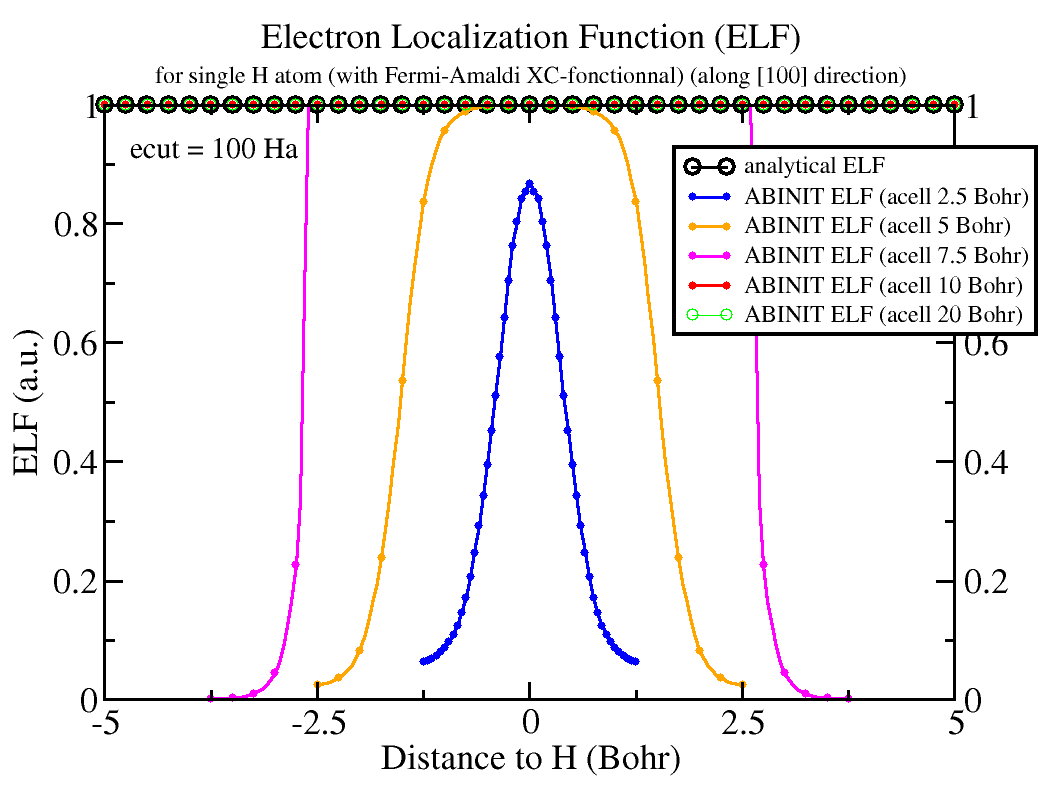
\includegraphics[width = \textwidth]{fig1}
\end{minipage}
\vspace{0.12\textwidth}
\begin{minipage}[c]{0.8\textwidth}
\caption{\small Comparison between analytical $ELF$ and ABINIT $ELF$ for an isolated H atom.}
\vspace*{1.0ex}
\label{fig1}
\end{minipage}
\end{figure}


Then the convergence with ecut parameter (Fig.(\ref{fig1})). The thing is that the convergence of $ELF$ seems to be more sensitive to the acell parameter than the ecut parameter, at least here for the hydrogen atom. For instance with only an ecut of $10$ Ha but with a $10$ Bohr box we already obtain $1$ everywhere.
\begin{figure}[!h]
\centering
\begin{minipage}[c]{1.0\textwidth}
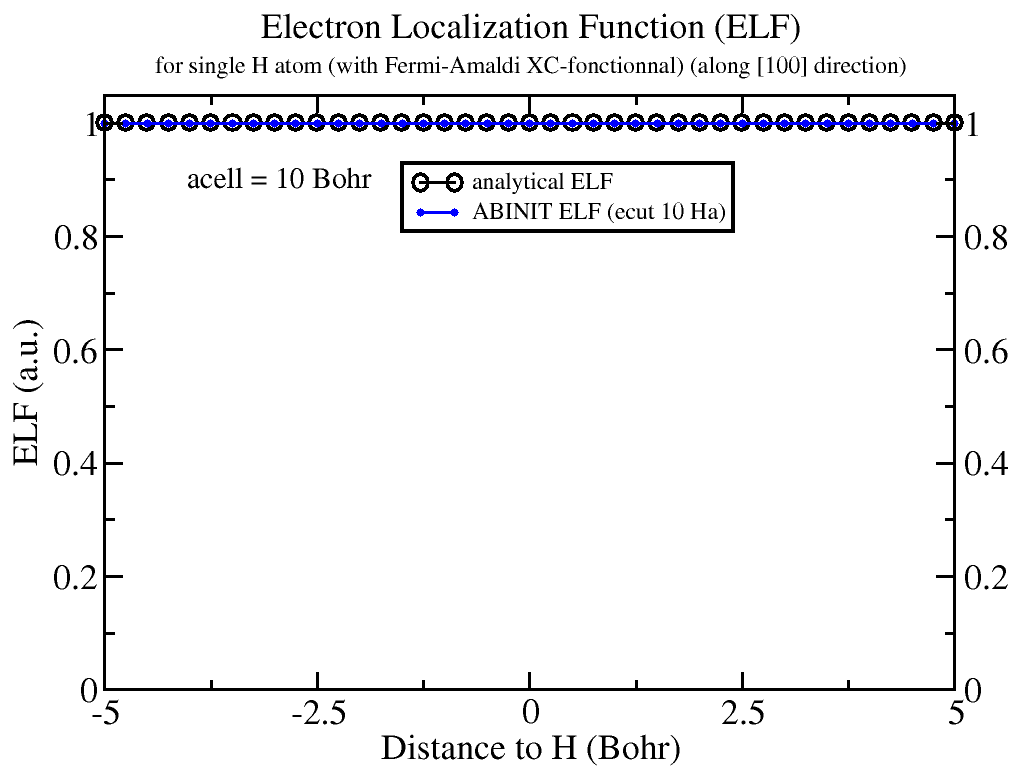
\includegraphics[width = \textwidth]{fig2}
\end{minipage}
\vspace{0.12\textwidth}
\begin{minipage}[c]{0.8\textwidth}
\caption{\small Comparison between analytical $ELF$ and ABINIT $ELF$ for an isolated H atom.}
\vspace*{1.0ex}
\label{fig1}
\end{minipage}
\end{figure}


\chapter{Test on an isolated Li atom.}
\label{chapter2}

Since the hydrogen atom is a bit peculiar for test of $ELF$ we have also performed a test with another isolated atom. We use here lithium (Li) because $ELF$ which can be used to show up the shell structure of isolated atoms, is very simple fo Li. Actually for Li this is just a single \textit{s} shell. We use for that an all electron calculation\footnote{the pseudopotential used is 03li.pspfhi and also a by-hand constructed bare pseudopotential 03li.bare}.

First with a bare pseudopotential (Fig.(\ref{fig3}) and Fig.(\ref{fig4})):

\begin{figure}[!h]
\centering
\begin{minipage}[c]{1.0\textwidth}
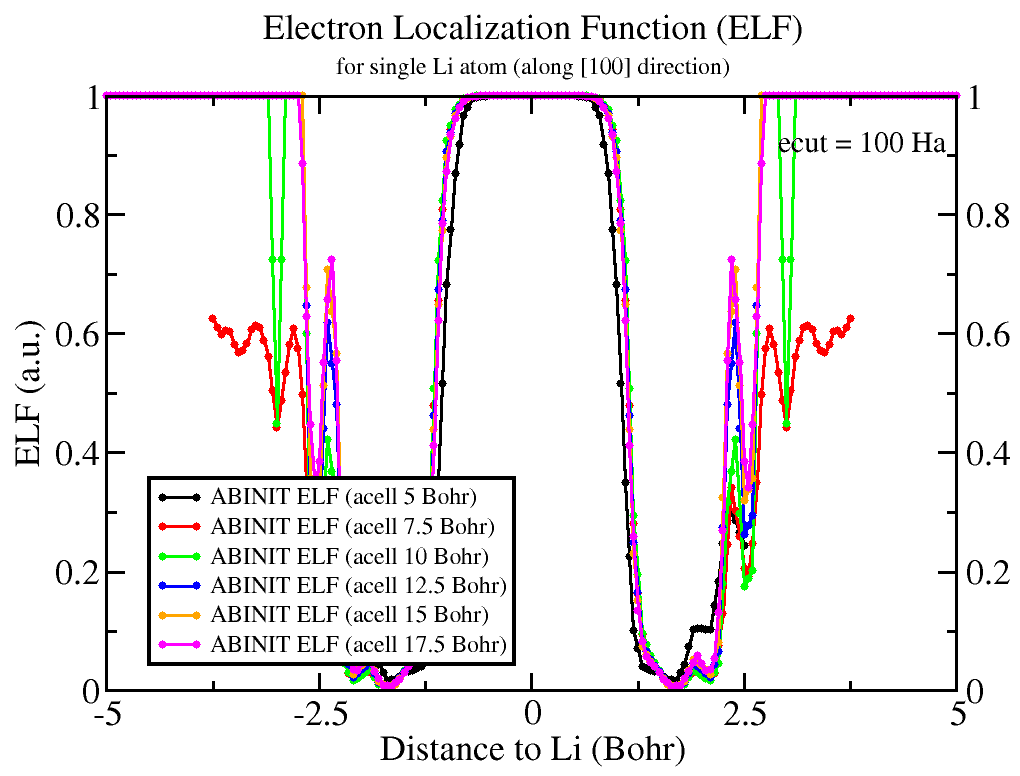
\includegraphics[width = \textwidth]{fig3}
\end{minipage}
\vspace{0.12\textwidth}
\begin{minipage}[c]{0.8\textwidth}
\caption{\small ABINIT $ELF$ for an isolated Li atom with a bare pseudo.}
\vspace*{1.0ex}
\label{fig3}
\end{minipage}
\end{figure}


\begin{figure}[!h]
\centering
\begin{minipage}[c]{1.0\textwidth}
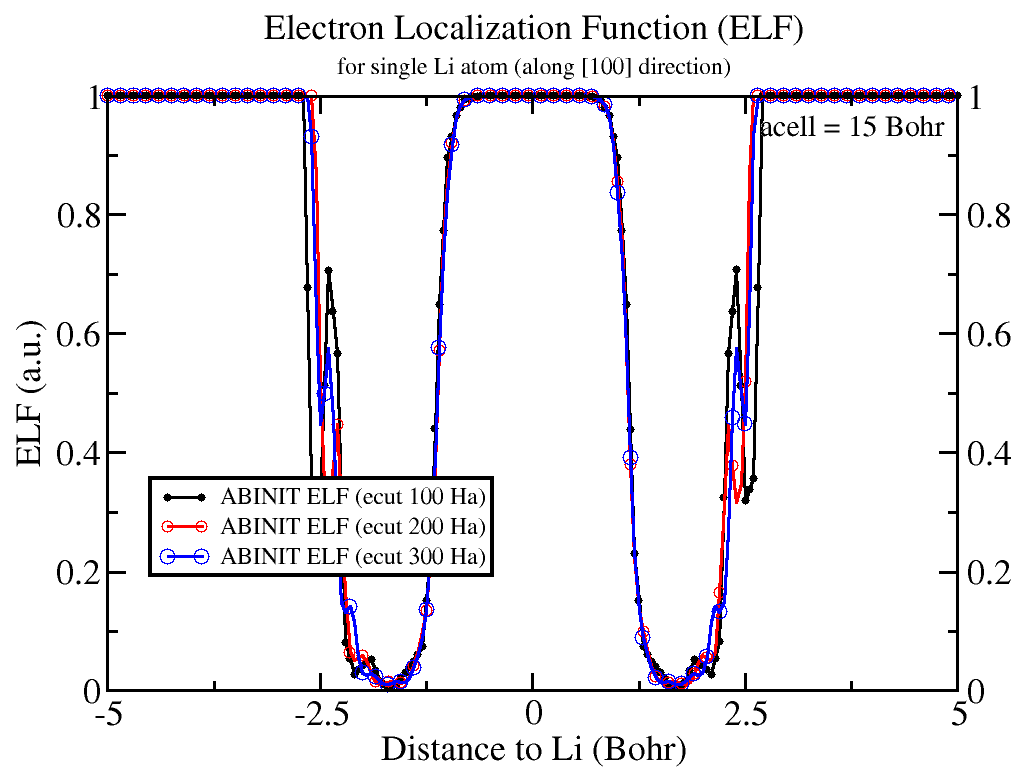
\includegraphics[width = \textwidth]{fig4}
\end{minipage}
\vspace{0.12\textwidth}
\begin{minipage}[c]{0.8\textwidth}
\caption{\small ABINIT $ELF$ for an isolated Li atom with a bare pseudo.}
\vspace*{1.0ex}
\label{fig4}
\end{minipage}
\end{figure}

Then with \textbf{fhi} pseudopotential (Fig.(\ref{fig5}) and Fig.(\ref{fig6})):

\begin{figure}[!h]
\centering
\begin{minipage}[c]{1.0\textwidth}
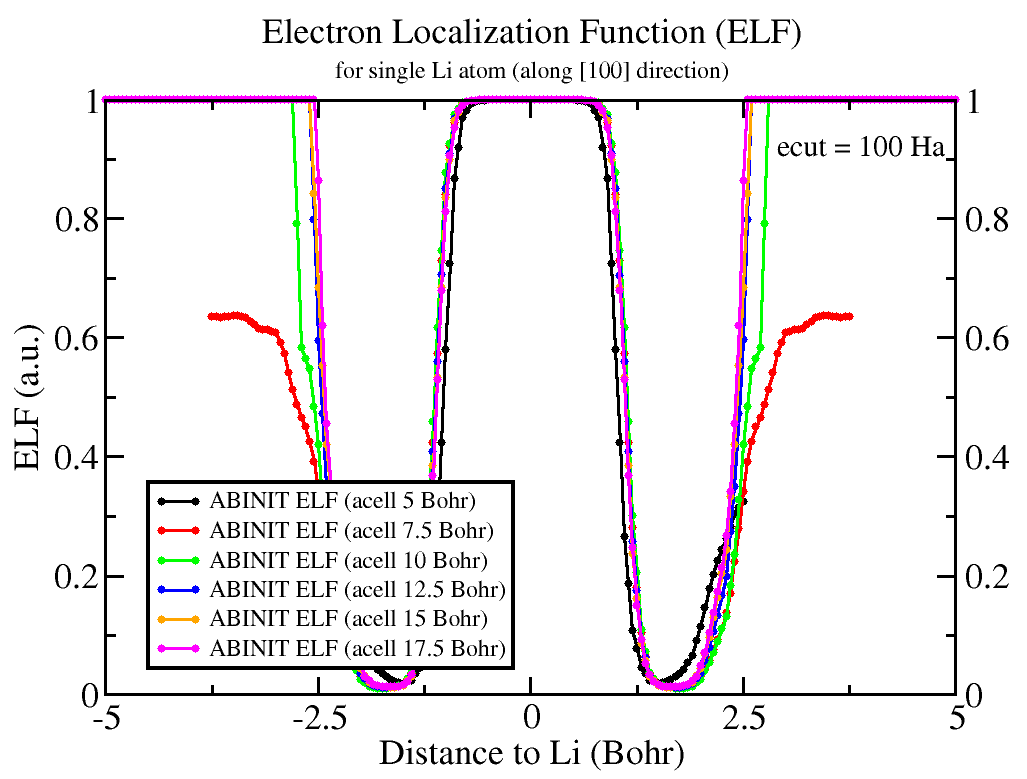
\includegraphics[width = \textwidth]{fig5}
\end{minipage}
\vspace{0.12\textwidth}
\begin{minipage}[c]{0.8\textwidth}
\caption{\small ABINIT $ELF$ for an isolated Li atom with a \textbf{fhi} pseudo.}
\vspace*{1.0ex}
\label{fig5}
\end{minipage}
\end{figure}

\begin{figure}[!h]
\centering
\begin{minipage}[c]{1.0\textwidth}
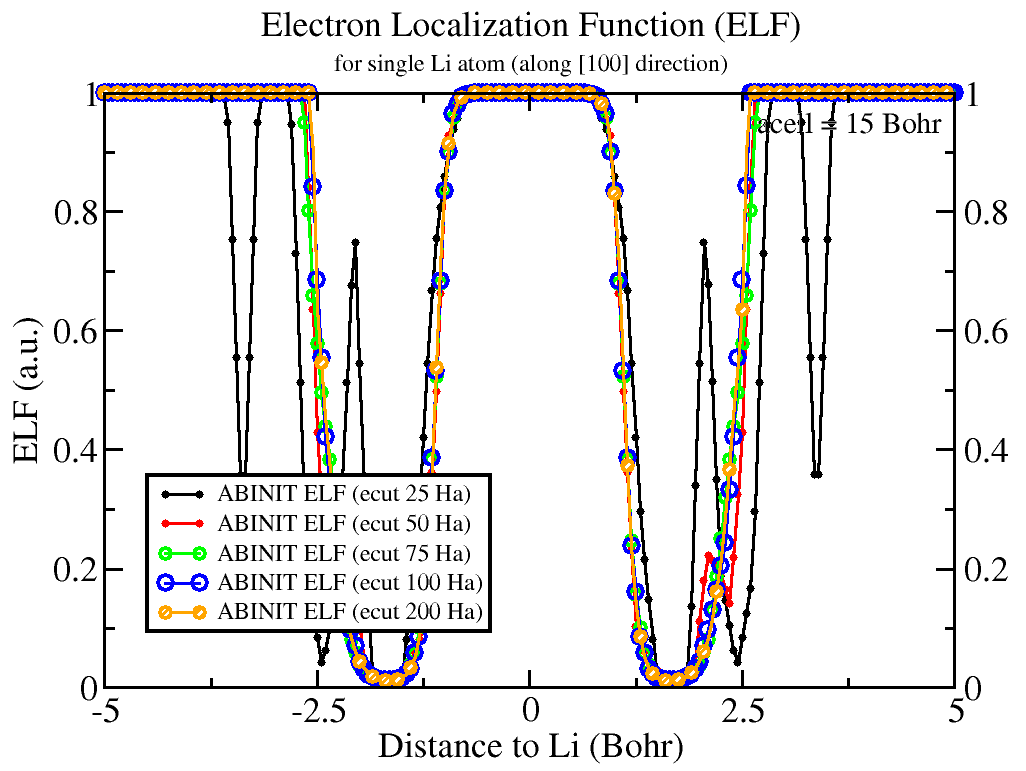
\includegraphics[width = \textwidth]{fig6}
\end{minipage}
\vspace{0.12\textwidth}
\begin{minipage}[c]{0.8\textwidth}
\caption{\small ABINIT $ELF$ for an isolated Li atom with a \textbf{fhi} pseudo.}
\vspace*{1.0ex}
\label{fig6}
\end{minipage}
\end{figure}

\end{document}
